\subsubsection{KNN Classifier}

During initial experimentation, KNN took over 22 hours to predict on the test set following training - Figure \ref{fig:knn_train}. Additionally, utilising the VM machine to train, KNN took over 28 hours to predict the test set of data, and subsequently crashed the system multiple times before results or evidence could be gathered. KNN's algorithm means it does not build and store a model during training but rather stores them in memory. As a result, when predicting on the test set, it required high computational power as KNN searches for the K-nearest neighbour from the training set. Due to a large number of features, this further increases the computational power required for these tasks. This was deemed too long for real-world applications where detecting network attacks would be time-sensitive. As network attacks can occur quickly, an IDS using ML algorithms needs to have a quick response to detect these attacks.

Therefore, despite the advantages of KNN, such as being easy to implement and interpret, the prioritisation of speed and accuracy in this work led to the ultimate decision not to continue with this classifier. Consequently, the results for this classifier remain inconclusive.

\medskip

\begin{figure}[h]
\caption{Training Time for KNN Classifier}
\label{fig:knn_train}
\centering
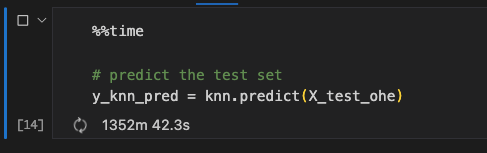
\includegraphics[width=\textwidth]{Appendices/Images/knn_predict-2023-04-15.png}
\end{figure}